Für die Fehlerrechung wird die empirische Standartabweichung
\begin{equation}
  \sigma = \sqrt{\frac{1}{n-1} \cdot \sum_{i=1}^n(x_i-\overline{x})^2}
  \label{eqn:Stdabweichung}
\end{equation}
und die Gaußsche Fehlerfortpflanzung
\begin{equation}
  u_y = \sqrt{\sum_{i=1}^n\left(\frac{\delta y}{\delta x_i}u_x\right)^2}
  \label{eqn:gauß}
\end{equation}
verwendet.
\begin{figure}
  \centering
  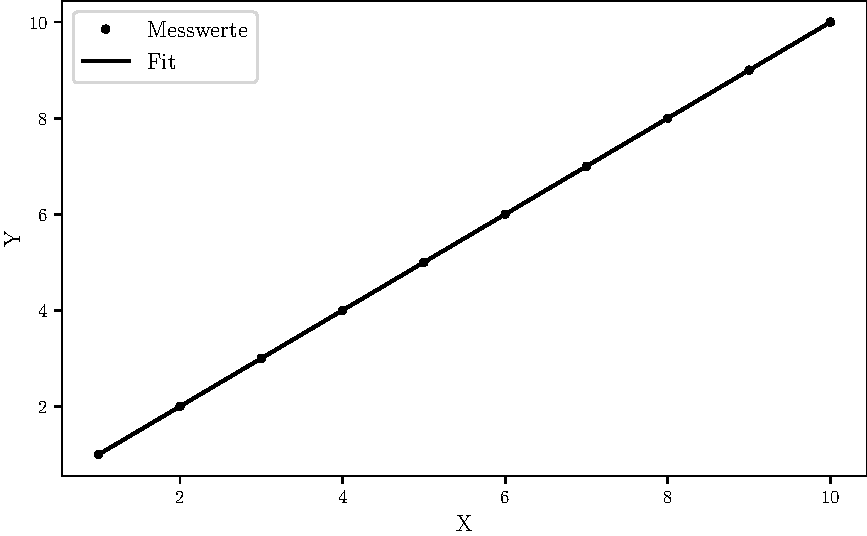
\includegraphics{build/plot.pdf}
  \caption{Plot}
  \label{fig:plot}
\end{figure}
